\chapter{Spatial variation of data characteristics}
\label{chap:spatial}
\begin{strip}
	\begin{minipage}{\textwidth}
		\begin{abstract}
			In the following chapter I present an analysis of variation of data characteristics by latitude and longitude. I find little correlation between data characteristics and latitude, and a limited correlation with longitude. However, I find supporting results for a model of diurnal shift. A symmetric distribution for meteor counts is suggested from the results.
		\end{abstract}
	\end{minipage}
\end{strip}
\section{Background}
The significance of this analysis includes a supporting argument for diurnal shift (see chapter~\ref{chap:diurnalshift}), and potential identification of locations with particularly good detection counts, which has implications for the levels of radio noise where the detection takes place. An analysis of detection rates based on both longitude and latitude could yield results that beg an investigation: perhaps at higher latitudes there are more meteors travelling tangential to the atmosphere, giving more detections.
\section{Literature Review}
Unfortunately, no literature existed regarding this subject. Well, there is now!
\section{Methodology}
In this chapter I present two analyses on the variation of certain data characteristics by latitude and longitude. In order to carry out these analyses, the observers from the RMOB data must be split into categories based on location.
\paragraph{Selecting observers\\}
Observers were selected based simply on whether they had Google Maps (GMAP) co-ordinates available. These co-ordinates are entered when uploading data to RMOB and are stored as part of the observer class location attributes dictionary. Provided an observer had {\it both} latitude and longitude available, then the analysis would be carried out on this data. Once all the observers had been checked and analysed (if necessary), the categorisation into groups could take place.
I used a basic process to group the observers, based on the difference between the current observer and the previous. The observers had to be sorted by increasing latitude or longitude (depending on the analysis) first. If the difference between co-ordinates was less than 10 degrees, then the two observers are considered part of the same group. This resulted in 9 categories for latitude, and 14 for longitude. These categories are not uniformly spread around the globe, but do provide a grouping of observers.
\paragraph{Analysis\\}
These characteristics summarise the data, namely 6 values: mean hourly count, max hourly count, skewness, peak hour of diurnal shift, fit to a sine function, and standard error. The standard error of all data for the observer is significant since it indicates how much the data varies over the time frame under consideration. A lower value indicates that the same detection count is generally seen, and a larger value indicates that the detection count varies erratically. The skew also indicates the distribution of the detection counts. A positive skew indicates that the detection counts trail off towards high values, whilst a negative skew indicates that the distribution is `steeper' for higher values, suggesting that there is a limit to the detection counts. The last two values are the peak hour of the diurnal shift, and the fit to an optimised sine curve for the mean detection counts over each hour of a day. This is calculated by averaging the values for all data for a given hour after midnight. A sine curve is in then fit to this, in the same process as chapter~\ref{chap:diurnalshift}, giving a sine function of the form $N = A \sin \left( \omega t + \phi \right) + \mu$ where $N$ is the detection count. The calculated `fit' is the sum of the standard deviations for $A$, $\mu$, and $\phi$. $\omega$ is assumed to be $\frac{2\pi}{24}$ so that the shift has a period of one day.
These 6 values will be calculated for each `entry' (month) for each observer, and then a mean will be taken from all the results for a given location category.

\section{Results}

\subsection{Latitude analysis}
\paragraph{Sample sizes \\}
Table~\ref{tab:spat:lat} shows the sample sizes for each latitude category.
\begin{table}[h!]
	\centering
	\begin{tabular}{ccc}
		\hline 
		Category & Latitude range ($^{\circ}$) & N$^o$ observers \\ 
		\hline 
		I & -43 -- -33 & 2 \\
		II & -31 -- -22 & 3 \\
		III & -20 -- -19 & 1 \\
		IV & -4 -- 5 & 3 \\
		V & 8 -- 12 & 2 \\
		VI & 23 -- 33 & 5 \\
		VII & 33 -- 44 & 33 \\
		VIII & 44 -- 53 & 107\\
		IX & 54 -- 57 & 9 \\  
		\hline
	\end{tabular} 
	\caption{Sample sizes for latitude categories \label{tab:spat:lat}}
\end{table}

\paragraph{Mean hourly detection count\\}
As can be seen in figure~\ref{fig:spat:lat:mean}, overall, the detection count is ${\sim}$ 60. There is a very low sample size for the category around a latitude of 0, which explains the large standard error. There does not appear to be an overall trend, there are no exceedingly anomalous results and there is no clear pattern across the categories. The minimum mean hourly detection count is category II (${\sim} -30^{\circ}$) and the maximum is (${\sim 0}^{\circ}$).
\begin{figure}[h!]
	\centering
	\includegraphics[width=\linewidth]{spatial/latitude/mean}
	\caption{Mean hourly detection count
		\label{fig:spat:lat:mean}}
\end{figure}
\paragraph{Maximum hourly detection count\\}
The standard errors are generally larger for the same categories compared to the mean hourly count. This suggests there is a much larger variation in the maximum count within each category. There is no clear trend over the latitude categories, as there is a large peak in category IV as well as VII. The lowest maximum hourly count is category III.
\begin{figure}[h!]
	\centering
	\includegraphics[width=\linewidth]{spatial/latitude/max}
	\caption{Maximum hourly detection count
		\label{fig:spat:lat:max}}
\end{figure}

\paragraph{Minimum hourly detection count\\}
For categories I--VI the minimum is 1. This is as expected. Category IX has the largest minimum, though there is a large error, indicating the low sample size. Categories VII--IX are the only categories without a minimum of 0. 
\begin{figure}[h!]
	\centering
	\includegraphics[width=\linewidth]{spatial/latitude/min}
	\caption{Minimum hourly detection count
		\label{fig:spat:lat:min}}
\end{figure}
\paragraph{Skewness\\}
Generally, the skewness is positive. There is a large error (relative to the values) indicating a widely varying skewness within each category. There is no clear trend, though the skewness {\it appears} to decrease as the latitude increases. There is only one category (V) with a negative skewness.
\begin{figure}[h!]
	\centering
	\includegraphics[width=\linewidth]{spatial/latitude/skew}
	\caption{Skewness of hourly counts
		\label{fig:spat:lat:skew}}
\end{figure}
\paragraph{Standard error\\}
The standard error appears to be relatively low for most of the categories, and with similar values, varying only by ${\sim}$ 3. The only exception to this is category IV, which has the largest standard error of ${\sim} 10$, though there is a much larger error in this than the other categories. This could simply be an anomalous reading.
\begin{figure}[h!]
	\centering
	\includegraphics[width=\linewidth]{spatial/latitude/err}
	\caption{Variation in hourly detection count 
		\label{fig:spat:lat:err}}
\end{figure}
\paragraph{Diurnal shift\\}
There is no clear trend for the peak hour of the diurnal shift. There is a large error for most categories, for all categories having at least an error of 1 hour. The large error indicates a large amount of variation within each category.
\begin{figure}[h!]
	\centering
	\includegraphics[width=\linewidth]{spatial/latitude/peak}
	\caption{Peak hour of diurnal shift
		\label{fig:spat:lat:peak}}
\end{figure}\\
For categories I--III and V, the fit is relatively good (${\sim}$ 2). Categories VI--IX have a slightly worse fit, around 6. Rather anomalously, category IV has a very poor fit, though in figure~\ref{fig:spat:lat:err} a large amount of variation is seen, so this is expected.
\begin{figure}[h!]
	\centering
	\includegraphics[width=\linewidth]{spatial/latitude/fit}
	\caption{Fit of diurnal shift to an optimal sine function
		\label{fig:spat:lat:fit}}
\end{figure}

\subsection{Longitude analysis}

\paragraph{Sample sizes\\}
Table~\ref{tab:spat:long} shows the sample sizes for each longitude category.
\begin{table}[h!]
	\centering
\begin{tabular}{ccc}
	\hline 
	Category & Longitude range ($^{\circ}$) & N$^o$ observers \\ 
	\hline 
	I & -123 -- -114 & 7 \\ 
	II & -112 -- -104 & 6 \\ 
	III & -100 -- -90 & 4 \\ 
	IV & -88 -- -78 & 4 \\ 
	V & -72 -- -71 & 1 \\ 
	VI & -48 -- -44 & 2 \\ 
	VII & -9 -- 0 & 56 \\ 
	VIII & 1 -- 12 & 32 \\ 
	IX & 12 -- 21 & 34 \\ 
	X & 22 -- 32 & 5 \\ 
	XI & 36 -- 46 & 4 \\ 
	XII & 47 -- 49 & 4 \\  
	XIII & 109 -- 110 & 1 \\ 
	XIV & 139 -- 148 & 3 \\  
	\hline
\end{tabular} 
\caption{Sample sizes for longitude categories \label{tab:spat:long}}
\end{table}

\paragraph{Mean hourly detection count\\}
There is no clear trend for the mean hourly count. The lowest mean is $|{\sim}$ 10, for category VI. The maximum is XII, with a mean hourly count of more than 200. The errors are smallest for the categories with the largest sample sizes, namely categories VII--IX.
\begin{figure}[h!]
	\centering
	\includegraphics[width=\linewidth]{spatial/longitude/mean}
	\caption{Mean hourly detection count
		\label{fig:spat:lon:mean}}
\end{figure}
\paragraph{Maximum hourly detection count\\}
Most maximum hourly detection counts are around 500, though there is an anomalous maximum for category X, with a maximum of more than 4000. This is likely only a single observer, however, as indicated by the low sample size and large error.
\begin{figure}[h!]
	\centering
	\includegraphics[width=\linewidth]{spatial/longitude/max}
	\caption{Maximum hourly detection count
		\label{fig:spat:lon:max}}
\end{figure}
\paragraph{Minimum hourly detection count\\}
The minimum values are, unlike in figure~\ref{fig:spat:lat:min}, not all 1. Most are a low value, though there is an anomalous result for XII, similar to the mean hourly count. This anomalous result is reflected by the large error.
\begin{figure}[h!]
	\centering
	\includegraphics[width=\linewidth]{spatial/longitude/min}
	\caption{Minimum hourly detection count 
		\label{fig:spat:long:min}}
\end{figure}
\paragraph{Skewness\\}
9 out of 14 categories are positive. This is similar to figure~\ref{fig:spat:lat:skew}. There is a large error for most categories, indicating a large amount of variation within each category. This suggests there is little correlation between longitude and skewness of hourly counts.
\begin{figure}[h!]
	\centering
	\includegraphics[width=\linewidth]{spatial/longitude/skew}
	\caption{Skewness of hourly counts
		\label{fig:spat:lon:skew}}
\end{figure}
\paragraph{Standard error\\}
Figure~\ref{fig:spat:lon:err} shows that there is a relatively low variation for most categories. The exceptions are categories X and XII, with errors of ${\sim 10}$ and ${\sim 15}$ respectively. There is a small error for all other categories, indicating a similar level of variation within the category.
\begin{figure}[h!]
	\centering
	\includegraphics[width=\linewidth]{spatial/longitude/err}
	\caption{Variation in hourly detection count
		\label{fig:spat:lon:err}}
\end{figure}
\paragraph{Diurnal shift\\}
There appears to be a correlation between longitude and the peak hour of diurnal shift. This is discussed in more detail in chapter~\ref{chap:diurnalshift}. The peak hour is lowest for low longitudes, around 6, and larger for large latitudes, approximately 14 for a longitude of -125$^{\circ}$ and 125$^{\circ}$.
\begin{figure}[h!]
	\centering
	\includegraphics[width=\linewidth]{spatial/longitude/peak}
	\caption{Peak hour of diurnal shift
		\label{fig:spat:lon:peak}}
\end{figure}\\
Generally, the fit is around ${\sim} 4$ for all categories other than IV, X, and XII. There are very poor fits for categories X and XII, though these categories have anomalous readings in other analyses too. Other than these two categories, the errors are small.
\begin{figure}[h!]
	\centering
	\includegraphics[width=\linewidth]{spatial/longitude/fit}
	\caption{Fit of diurnal shift to an optimal sine function
		\label{fig:spat:lon:fit}}
\end{figure}

\section{Discussion}
\subsection{Latitude analysis}
\paragraph{Mean, maximum \& minimum hourly count\\}
The mean does not appear to correlate with the latitude, but this is expected. Though the aim of this analysis was to determine if there are especially good locations for meteor detection, the reality is that on average, most places will be of the same quality for meteor detection. \\
It is not necessarily expected that the minimum {\it isn't} 1, though the reason is likely that most observers in the category {\it do} have a minimum of 1, but a few observers don't, which changes the mean minimum. This is a reasonable explanation, since the only categories that don't have a mean minimum of 1 have the largest sample sizes.
Larger variations in maximum are expected. The maximum has no limit (theoretically) though the minimum cannot be below 0, so variation in minimum is limited but this is not the case for maximum hourly detection counts.
\paragraph{Skewness\\}
The positive skewness is expected. There is likely to be more positive skew than negative, so on average it will be positive. Though most values are positive, they are all close to 0. This suggests that the distribution of meteor counts is symmetric.
\paragraph{Standard error\\}
There appears to be, on average, a small amount of variation in hourly counts. This was not expected: often counts may vary widely across the course of a day, though the range over which the variation takes place is apparently small enough that the standard error is not large.
\paragraph{Diurnal shift\\}
Correlation between latitude and the peak hour of an observer's diurnal shift is not expected, and this is reflected in the results. There is no apparent reason why the diurnal shift would vary with latitude, as discussed in chapter~\ref{chap:diurnalshift}.
\subsection{Longitude analysis}
\paragraph{Mean, maximum \& minimum hourly count\\}
There is no expectation for a correlation between the mean and the longitude. There is a large variation in the results, though without an analysis of location based on latitude {\it and} longitude, there is no way of knowing if the increased mean hourly detection counts are a result of the location or an observer's detection system.
\paragraph{Skewness\\}
Similar to the latitude analysis of skew, there is less grouping around 0 than expected. However, a slightly positive skew is not anomalous: counts will trail off towards larger numbers, but will never be below 0, giving a slightly positive skew.
\paragraph{Standard error\\}
The large increase in standard error for categories X and XII are obscure. This increase could be due to the location, but most likely it is a result of the set up of the observers in the sample. This would explain the anomalous results, since the low sample sizes of 5 and 4 respectively would allow for a large variation due to a single observer's counts.
\paragraph{Diurnal shift\\}
The apparent correlation between longitude and peak hour of diurnal shift is discussed in detail in chapter~\ref{chap:diurnalshift}. It is an expected result based on the model for diurnal shift.
\subsection{Improvements}
\paragraph{Percentiles\\}
Analysing the maximum and minimum hourly detection counts can only reveal a certain amount of information. It does give {\it some} indication towards the distribution of hourly counts, but taking quartiles, or 90th and 10th percentiles, will give more indication. The maximum may be extremely large, but there are no other values similar to it for a given observer, in which case the 90th percentile would reveal a lot more about the distribution. Similarly, the minimum is likely to always be 0 or 1, which does not provide much information, whilst the 10th percentile would indicate how many hourly counts are this small.
\paragraph{Joint latitude \& longitude analysis\\}
Whilst analysing latitude and longitude individually reveals, or thwarts, correlations, it is not as valuable as a joint analysis. This could be represented using a 3D plot, and would indicate much more clearly hotspots for meteor detection, and may reveal correlations that are not solely between latitude and longitude, but a correlation between the two.

\section{Conclusion}
There does not appear to be a large degree of correlation between most data characteristics and latitude or longitude. There appears to be a correlation between peak hour of diurnal shift and longitude, as expected based on the models discussed in chapter~\ref{chap:diurnalshift}. There are clearly anomalous readings for some results, namely standard error (longitude) and minimum hourly detection count (latitude). Likely explanations for this are low sample sizes. Further work, focusing on longitude and latitude, may clarify some results, indicating which apparent trends persist and which are anomalous.